\chapter{Solução Proposta} \label{cap:solucao}

Em resposta aos problemas identificados para processar as informações geradas pela estação meteorológica da EST e geração dos boletins meteorológicos, este trabalho se propôs a projetar e implementar uma plataforma web para gerenciamento de dados e geração de boletins meteorológicos do LabInstru. As seções a seguir apresentam artefatos resultantes da análise do problema e da concepção da solução proposta, detalhando os elementos que a caracterizam.


\section{Processo de Desenvolvimento Adotado}
O AUP foi escolhido como modelo de processo de desenvolvimento por seguir a metodologia ágil e por possuir diversos elementos que capturam a realidade do contexto em que este trabalho de conclusão de curso está sendo desenvolvido. Além dos elementos mencionados, um outro fator prepoderante para escolha do AUP foi o fato do software  desenvolvido não ser de grande porte e possuir uma equipe pequena de desenvolvimento, nesse caso, composta apenas de uma pessoa -- o aluno.

A Profa. Maria Betânia Leal exerceu o papel de cliente final da aplicação. O papel de solicitante do software foi exercido pela Profa. Elloá B. Guedes, a qual forneceu \emph{feedback} e auxiliou na validação das funcionalidades desenvolvidas.

Por estar baseado em uma abordagem iterativa e incremental, o AUP auxiliou a organização deste trabalho em séries de pequenas iterações, que puderam ser efetuadas levando em consideração um caso de uso por vez. Desta maneira, teve-se sempre um sistema parcial executável e testável, em que as partes desenvolvidas puderam ser facilmente integradas.

Em relação à algumas disciplinas do AUP, algumas decisões foram consideradas. Em termos de testes, foram considerados os testes feitos pelo próprio desenvolvedor utilizando os recursos disponíveis na linguagem de programação adotada, tal como o comando \texttt{assert}. O gerenciamento de configuração será efetuado com o auxílio das ferramentas Google Drive e Git para gerenciamento de documentos e de código, respectivamente. A disciplina de gerenciamento de projetos foi liderada pela profa. Elloá B. Guedes, que promoveu reuniões com a cliente sempre que necessário e estabeleceu prazos, atividades e marcos de entrega de acordo com o planejamento semestral do trabalho de conclusão de curso.


\section{Diagramas de Caso de Uso}
Após conversas com a cliente e com a solicitante do software, foi possível identificar quatro módulos principais que contemplam as diferentes funcionalidades solicitadas. Estes módulos são apresentados a seguir:

\begin{enumerate}
	\item \textbf{Módulo Gerencia Conta de Usuário}. Neste módulo, cujo ator principal é o administrador do sistema, concentram-se as funcionalidades relativas à manutenção de usuários, ilustradas no diagrama de caso de uso da Figura \ref{fig:casoUso1}. No cenário em que a plataforma será utilizada, foi possível identificar que não deve haver livre cadastro e acesso aos dados de maneira deliberada, daí a necessidade de um administrador para cadastrar novos usuários, que podem ser alunos de iniciação científica, pesquisadores, docentes, dentre outros;
	\begin{figure}[H]
		\centering
		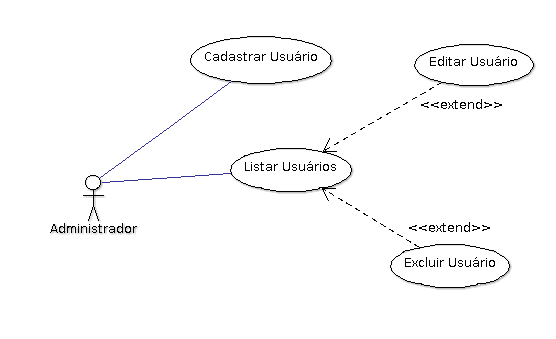
\includegraphics[scale=0.8]{img/uc001.png}
		\caption{Caso de Uso - Módulo Gerencia Conta de Usuário.}
		\label{fig:casoUso1}
	\end{figure}
	\item \textbf{Módulo Usuário}. Neste módulo, cujo ator principal é o usuário, encontram-se as funcionalidades relativas à manutenção dos dados do próprio usuário. Pode haver alterações de dados do perfil, redefinição e recuperação de senha, conforme ilustrado na Figura \ref{fig:casoUso2};
	\begin{figure}[H]
		\centering
		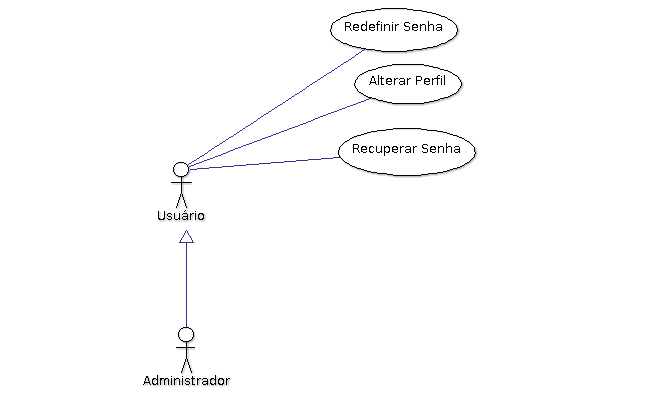
\includegraphics[scale=0.8]{img/uc002.png}
		\caption{Caso de Uso - Módulo Usuário.}
		\label{fig:casoUso2}
	\end{figure}
	\item \textbf{Módulo Consulta Medições}. Este módulo concentra as funcionalidades de acesso aos dados das estações. Conforme ilustra a Figura \ref{fig:casoUso3}, podem ser feitas consultas diretas aos dados, consulta à disponibilidade dos dados em um determinado mês e também aspectos da visualização dos dados, seja por meio de boletins como também por meio de gráficos, além da possibilidade de exportação. Estas funcionalidades foram identificadas considerando as principais solicitações de dados feitas por terceiros ao LabInstru;
	% figura 3
	\begin{figure}[H]
		\centering
		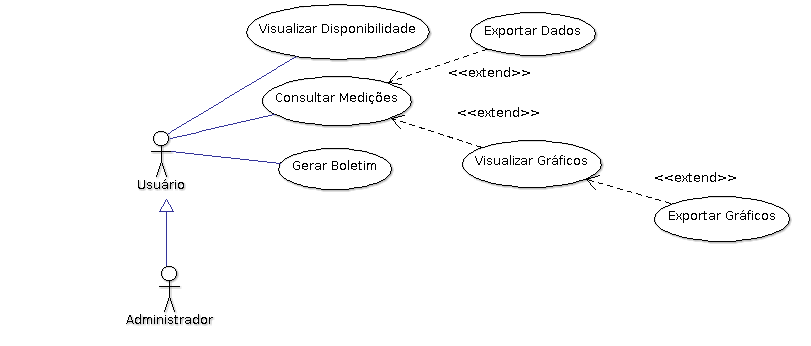
\includegraphics[scale=0.8]{img/uc003.png}
		\caption{Caso de Uso - Módulo Consulta Medições.}
		\label{fig:casoUso3}
	\end{figure}
	\item \textbf{Módulo Gerencia Medições}. O módulo de gerenciamento de medições permite que o administrador do sistema mantenha as medições do sistema a partir dos dados obtidos das estações meteorológicas do LabInstru. Considerando a importância de assegurar a origem destes dados e a remoção das eventuais medições inconsistentes, apenas o administrador está habilitado para execução das funcionalidades deste módulo, conforme ilustrado na Figura \ref{fig:casoUso4}.
	% figura 4
	\begin{figure}[H]
		\centering
		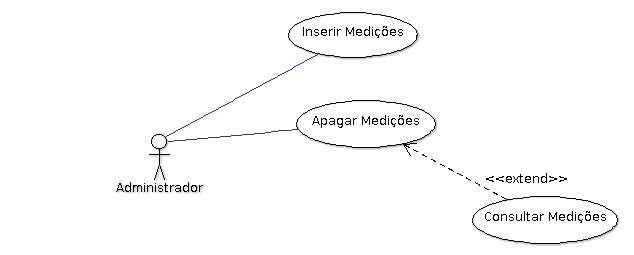
\includegraphics[scale=0.8]{img/uc004.png}
		\caption{Caso de Uso - Módulo Gerencia Medições.}
		\label{fig:casoUso4}
	\end{figure}
\end{enumerate}

O detalhamento de todos os casos de uso ilustrados nas Figuras \ref{fig:casoUso1}-\ref{fig:casoUso4} encontra-se disponível no Apêndice \ref{sec:aprendiceCasoUso},  onde podem ser vistos os interessados, pré e pós condições, fluxo principal, fluxo alternativo e regras de negócio.


\section{Modelo Conceitual}
Após a documentação dos requisitos funcionais e não funcionais sob a forma de casos de uso, foi possível obter um melhor entendimento do que deveria ser desenvolvido. Com a conclusão desta etapa, partiu-se para a elaboração do modelo conceitual, visando representar, em alto nível, as abstrações efetuadas e as associações entre elas. O modelo conceitual resultante é ilustrado na Figura \ref{fig:modeloConceitual}.

\begin{figure}[H]
	\centering
	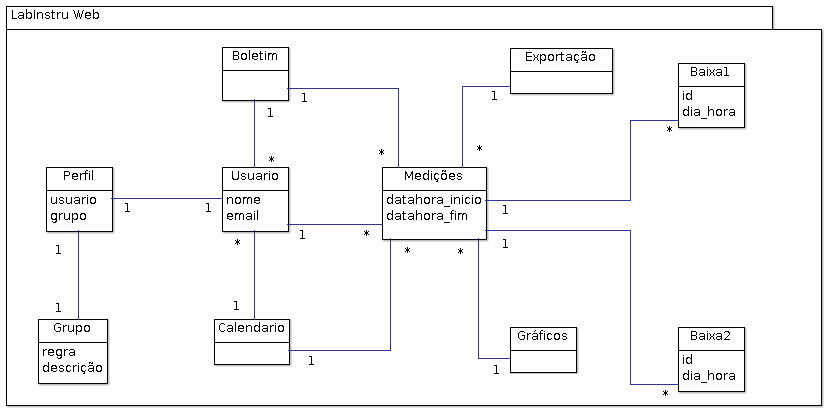
\includegraphics[scale=0.8]{img/ModeloConceitual.png}
	\caption{Módelo Conceitual - LabInstru Web.}
	\label{fig:modeloConceitual}
\end{figure}

Neste modelo, a entidade \texttt{Usuário} representa os atores que irão interagir com a aplicação. Cada usuário é encapsulado em um \texttt{Perfil} e os perfis são organizados em um \texttt{Grupo}, que contém um conjunto de regras e descrições. Há dois perfis de usuários: \texttt{Admin}, que possui os privilégios especiais de cadastrar novas medições provenientes da estação meteorológica da EST e manter os usuários; e \texttt{User}, grupo elementar, que utiliza as funcionaldiades disponibilizadas pela aplicação, tais como consulta às medições, exportação de dados, geração de boletins meteorológicos, dentre outras. É interessante notar que, embora não ressaltado neste modelo, todo \texttt{Admin} é um \texttt{User}.

Em relação aos dados meteorológicos da aplicação, estes são organizados em \texttt{Medições}, que podem conter dados oriundos do \texttt{Baixa1} ou \texttt{Baixa2}, advindos de dois tipos de arquivos distintos da estação meteorológica da EST. Em virtude deste ser um modelo de alto-nível, os atributos particulares que diferenciam e caracterizam o \texttt{Baixa1} e o \texttt{Baixa2} não estão detalhados.

Com entidadas do tipo \texttt{Medição}, os usuários podem então gerar um boletim meteorológico (\texttt{Boletim}), visualizar o calendário de disponibilidade (\texttt{Calendario}), gerar gráficos (\texttt{Gráficos}) ou exportar os dados produzidos (\texttt{Exportação}).

As ideias fundamentais contidas neste modelo conceitual serviram como ponto de partida para a elaboração dos elementos posteriores, detalhados nas seções a seguir.


\section{Prototipação das Telas do Usuário}
Considerando as funcionalidades identificadas e documentadas, partiu-se para elaboração de protótipos. Estes protótipos foram construidos considerando as principais funcionalidades a serem desenvolvidas, com o intuito de mostrar à cliente uma representação limitada da solução proposta, mas que permitisse explorar a sua conveniência. O resultado desta prototipação é mostrado a seguir. Embora os protótipos de todas as funcionalidades tenham sido elaborados, apenas os mais relevantes serão mostrados a seguir. Para elaborá-los foi utilizado o software Balsamiq Mockups \cite{Prototipacao:Mockups}.

A tela inicial da aplicação encontra-se ilustrada na Figura  \ref{fig:tela002}. No canto superior direito, há um link para o formulário de autenticação no sistema e também para recuperação de senha, caso algum usuário tenha esquecido da mesma.

\begin{figure}[H]
	\centering
	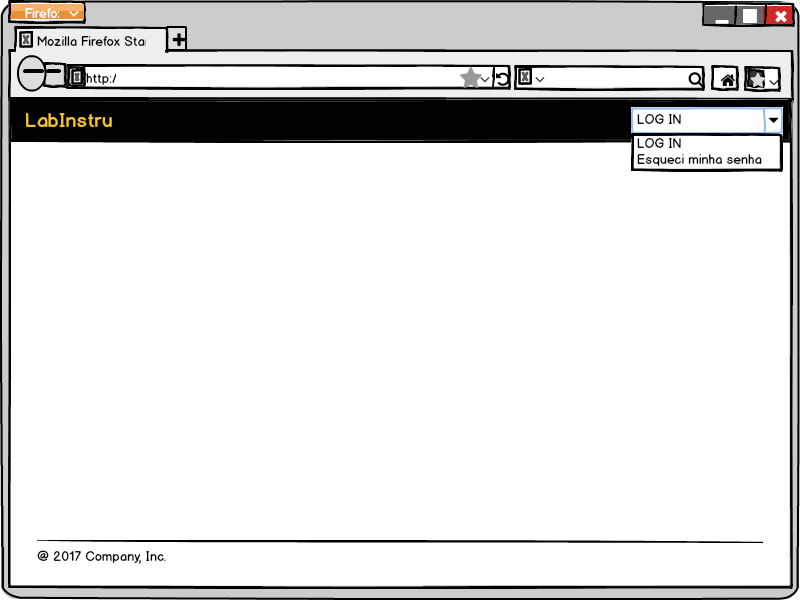
\includegraphics[width=0.8\textwidth]{./img/telas/tela002.png}
	\caption{Tela inicial da aplicação web LabInstru.} \label{fig:tela002}
\end{figure}

Considerando a perspectiva do usuário Administrador, o menu principal da aplicação disponível para o mesmo é mostrado na Figura \ref{fig:tela025}, no qual é possível selecionar a opção ``Cadastrar Usuário'' na aba ``Administração''.  Para efetuar a inclusão de um novo usuário na base de dados, o administrador será redirecionado para o formulário de cadastro ilustrado na Figura \ref{fig:tela027}.


\begin{figure}[H]
	\centering
	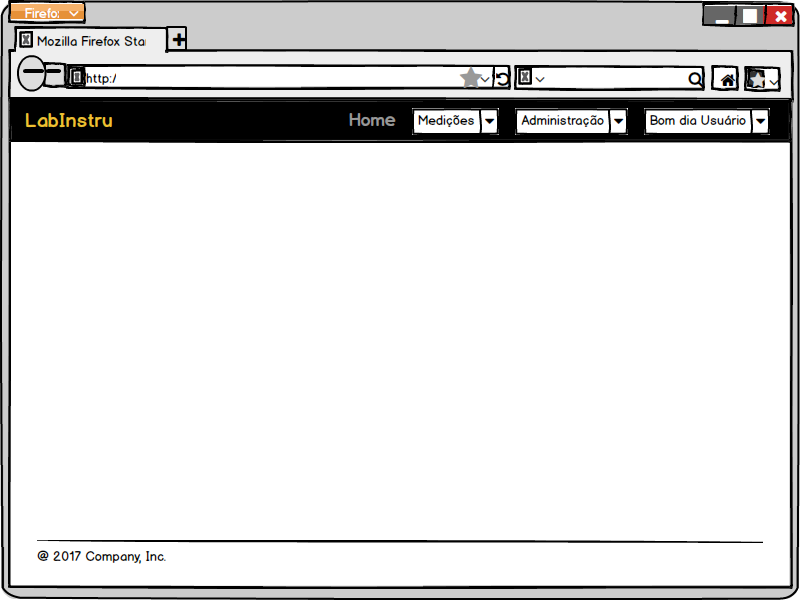
\includegraphics[width=0.8\textwidth]{./img/telas/tela025.png}
	\caption{Protótipo de tela do menu principal da aplicação.} \label{fig:tela025}
\end{figure}


\begin{figure}[H]
	\centering
	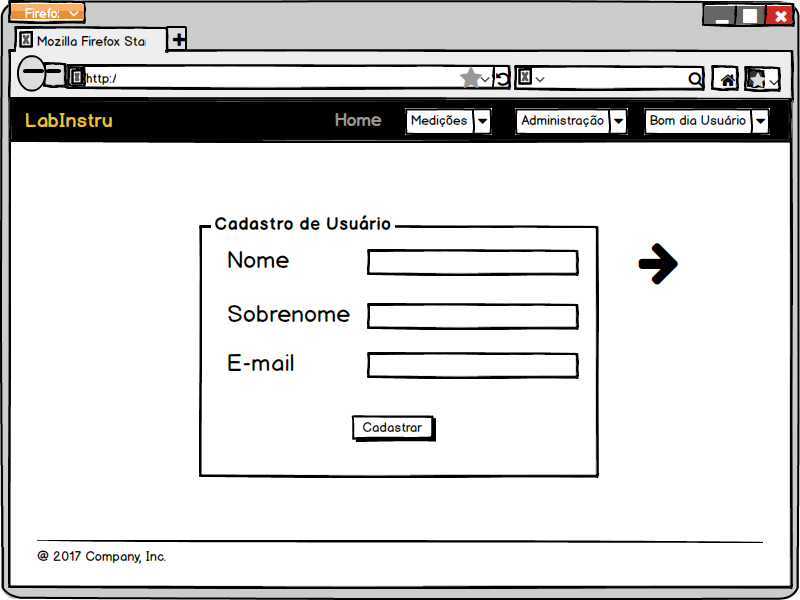
\includegraphics[width=0.8\textwidth]{./img/telas/tela027.png}
	\caption{Protótipo de tela referente ao cadastrado de usuário.} \label{fig:tela027}
\end{figure}

Para exibe uma listagem dos usuários cadastrados na base de dados da aplicação, e posteriormente, caso desejável, fazer a edição ou remoção de um usuário específico, deve-se esoclher a opção ``Listar Usuários'' na aba ``Administração'' do menu principal da aplicação, conforme Figura \ref{fig:tela033}.

\begin{figure}[H]
	\centering
	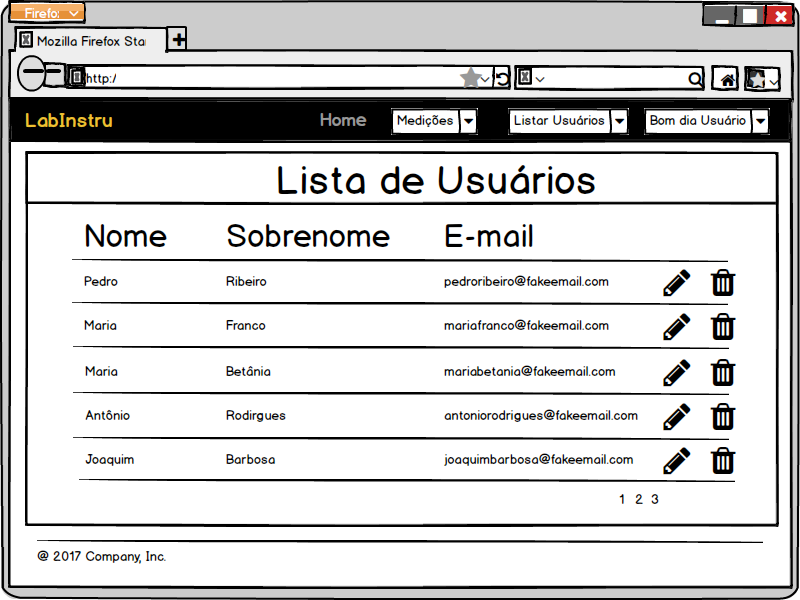
\includegraphics[width=0.8\textwidth]{./img/telas/tela033.png}
	\caption{Protótipo de tela referente à listagem de usuários.} \label{fig:tela033}
\end{figure}

O cadastro de novas medições é efetuado pelo Administrador. Para tanto, este deve utilizar um formulário análogo ao mostrado na Figura \ref{fig:tela053}, em que este deve fornecer um arquivo oriundo da estação meteorológia no formato \texttt{.dat}.

\begin{figure}[H]
	\centering
	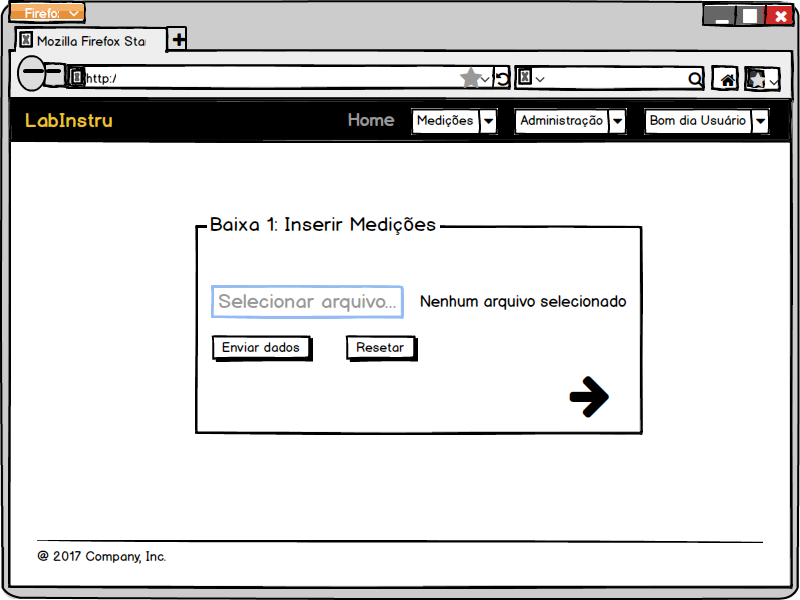
\includegraphics[width=0.8\textwidth]{./img/telas/tela053.png}
	\caption{Protótipo de tela para cadastro de novas medições.} \label{fig:tela053}
\end{figure}

Caso um usuário deseje efetuar uma consulta na base de dados, um formulário detalhado será exibido, conforme ilustrado na Figura  \ref{fig:tela058}, no qual o usuário deve informar os parâmetros para consulta dos dados. Ao submeter a consulta, as respostas serão exibidas conforme ilustrado na Figura \ref{fig:tela062}.

\begin{figure}[H]
	\centering
	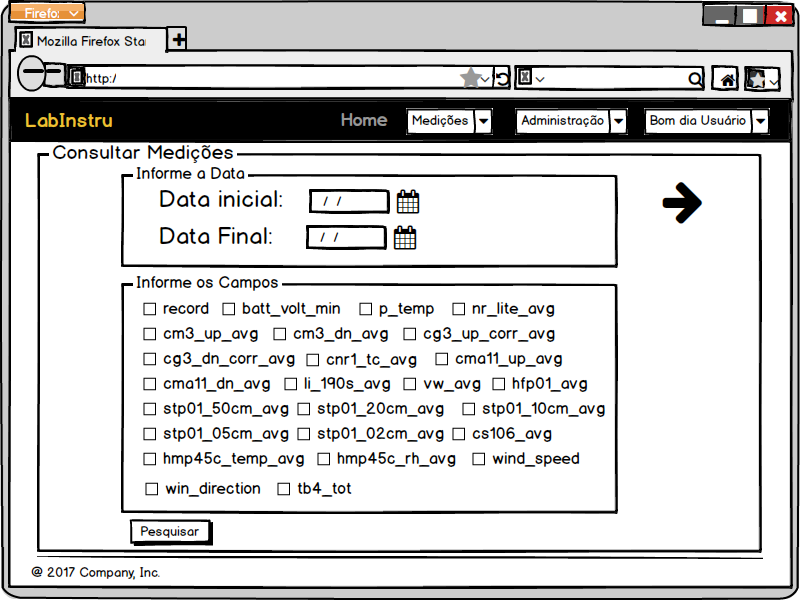
\includegraphics[width=0.8\textwidth]{./img/telas/tela058.png}
	\caption{Protótipo de tela referente ao formulário para consultar medições.} \label{fig:tela058}
\end{figure}

\begin{figure}[H]
	\centering
	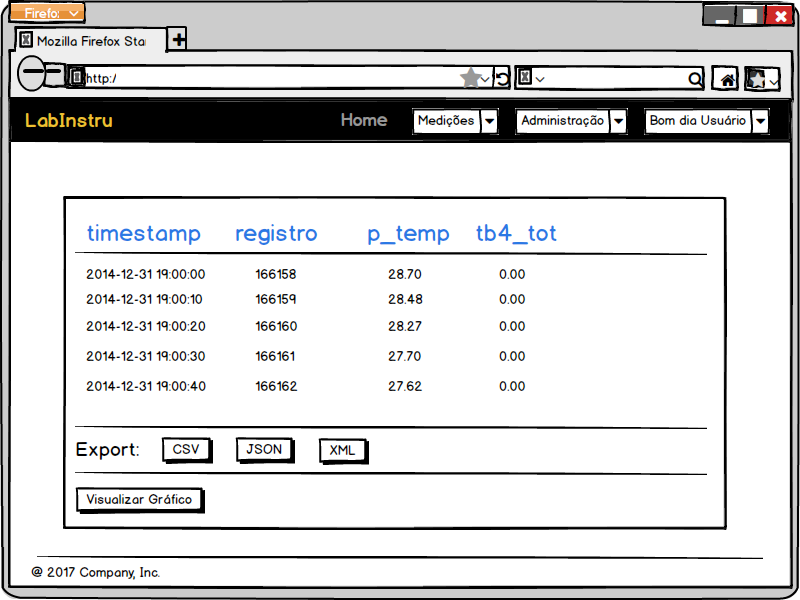
\includegraphics[width=0.8\textwidth]{./img/telas/tela062.png}
	\caption{Protótipo de tela referente à visão de saída a uma consulta de medições.} \label{fig:tela062}
\end{figure}

Por meio do menu principal da aplicação, escolhendo a opção disponibilidade, pertecente à aba de uma determinada estação meteorológica (Baixa 1 ou Baixa 2), vide Figura \ref{fig:tela072}, é possível ter acesso ao calendário de disponibilidade de medições diárias desta estação meteorológica. Esse calendário, conforme ilustrado na Figura \ref{fig:tela073}, tem por objetivo informar quantas medições estão disponíveis em todos os dias do mês escolhido, por meio de cores apropriadas.

\begin{figure}[H]
	\centering
	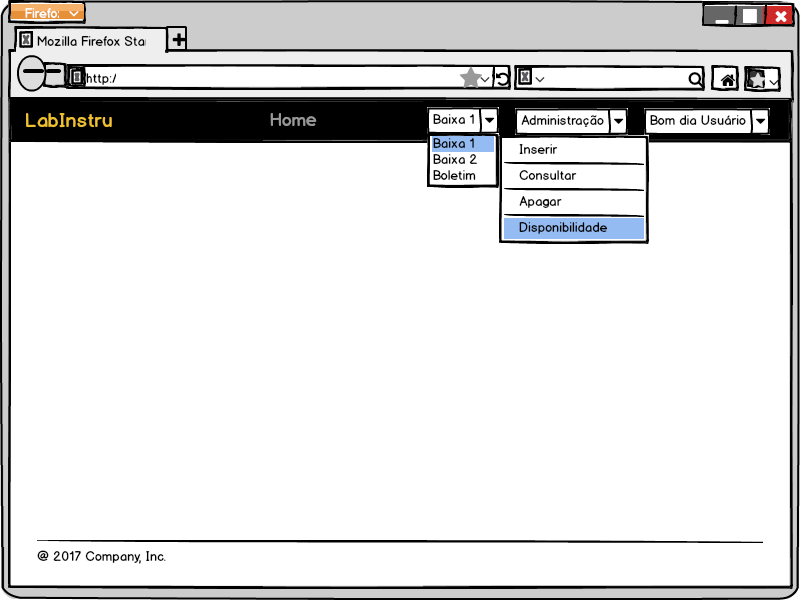
\includegraphics[width=0.8\textwidth]{./img/telas/tela072.png}
	\caption{Navegando no menu para funcionalidade Disponibilidade.} \label{fig:tela072}
\end{figure}

\begin{figure}[H]
	\centering
	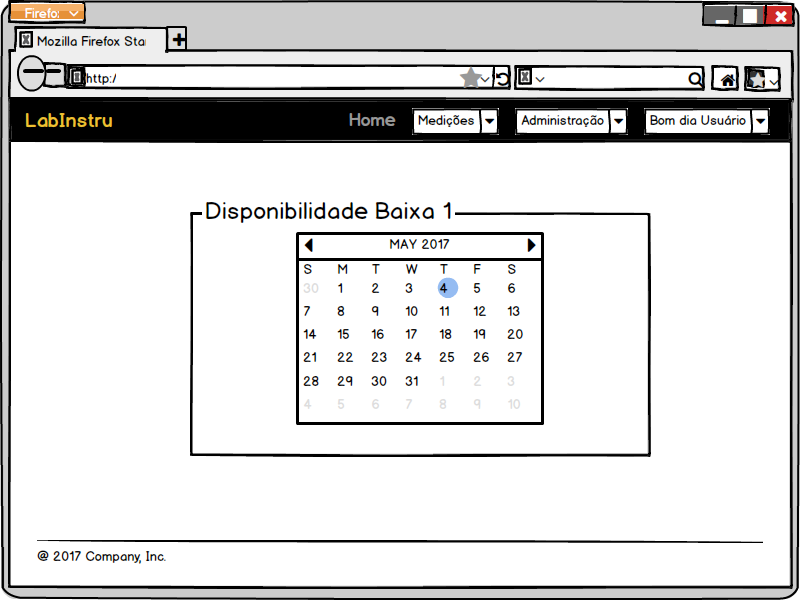
\includegraphics[width=0.8\textwidth]{./img/telas/tela073.png}
	\caption{Tela responsável por exibir o calendário de disponibilidade.} \label{fig:tela073}
\end{figure}

Outra funcionalidade importante na aplicação é o \textit{Boletim Meteorológico}, que pode ser acessado por meio da opção \textit{``Boletim''}, na aba \textit{``Medições''} do menu principal da aplicação. Esse boletim informará diversos dados meteorológicos (temperatura máxima, mínima, índice de calor, etc.) por dia de um determinado mês. A Figura \ref{fig:tela077} ilustra um exemplo de processamento resultante desta funcionalidade.

\begin{figure}[H]
	\centering
	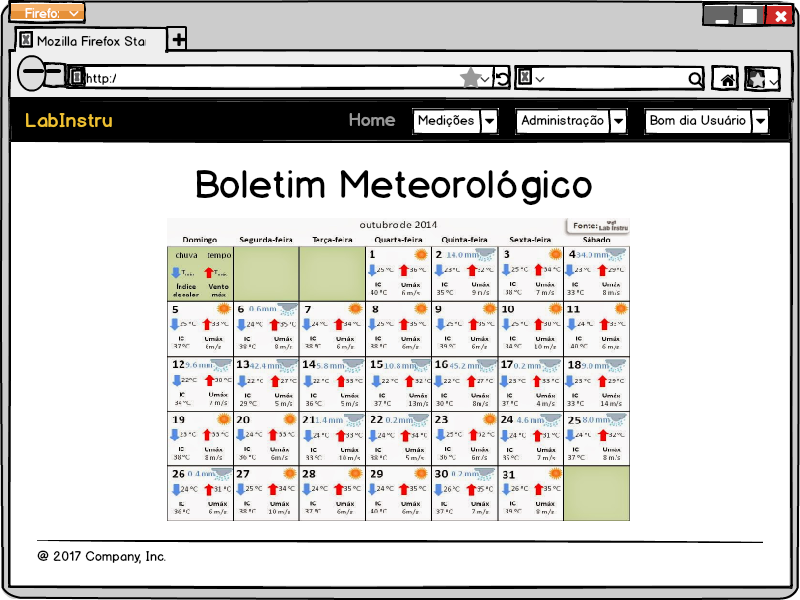
\includegraphics[width=0.8\textwidth]{./img/telas/tela077.png}
	\caption{Protótipo de tela responsável por mostrar o resultado do boletim meteorológico.} \label{fig:tela077}
\end{figure}


\section{Tecnologias Utilizadas}
As tecnologias utilizadas para elaboração da solução proposta consistem no \emph{framework} Web2py, detalhado anteriormente na Seção \ref{sec:web2py}, nos \emph{frameworks} Bootstrap, na biblioteca JQuery e no sistema gerenciador de banco de dados MySQL. Uma visão geral de cada uma dessas tecnologias será apresentado a seguir.

O Bootstrap é um \emph{framework} JavaScript, HTML e CSS para desenvolvimento de sites e aplicações web responsivas, possibilitando uma maior agilidade e facilidade no desenvolvimento do \emph{front-end} \cite{Silva:Livro}. Embora o Web2py utilize internamente este \emph{framework} para geração das \emph{views}, a utilização direta do Bootstrap no contexto deste trabalho foi necessária para proporcionar uma melhor customização das páginas web da  aplicação, resultando em um melhor dominio sobre as funcionalidades envolvidas nas páginas web.

O JQuery é uma biblioteca JavaScript que simplifica a manipulação de documentos HTML, eventos, animações e interações AJAX no desenvolvimento rápido de aplicações web \cite{Duckett:JS}. Assim como no caso do Bootstrap, o Web2py também faz uso interno desta biblioteca, porém a manipulação direta da mesma provê  uma melhor customização e controle das funcionalidades, considerando a adição de efeitos visuais, melhoria de aspectos de interatividade e simplificação de determinadas tarefas, razão pela qual considerou-se também a demanda por JQuery no contexto deste trabalho.

Como mencionado anteriormente, o \emph{framework} Web2py já possui o banco de dados SQLite integrado. Porém, este banco de dados possui algumas limitações de desempenho, razão pela qual optou-se pela adoção do MySQL, um sistema gerenciador de banco de dados considerado versátil e com suporte a diversas plataformas e diferentes linguagens, bastante utilizado em aplicações web e desktop \cite{MySql:MySql}. Para facilitar a administração do banco de dados, a ferramenta MySQL Workbench \cite{MySql:WorkBench} também foi utilizada, visando prover auxílio na visualização dos dados do banco, realizar testes e gerenciar as mudanças.


\section{Apresentação da Plataforma}
O \emph{LabInstru Web}, nome dado à plataforma desenvolvida no escopo deste trabalho de conclusão de curso, é o resultado da implementação das funcionalidades identificadas e prototipadas nas etapas anteriores. Esta plataforma foi desenvolvida utilizando o \emph{framework} Web2py, banco de dados MySQL e tecnologias como JQuery e Bootstrap. A página inicial da aplicação encontra-se ilustrada na Figura \ref{fig:ap1}. A partir da página principal da aplicação, é possível aos seus usuários utilizarem as funcionalidades para autenticação no sistema, vide Figura \ref{fig:ap10}, bem como para recuperação de senha, vide Figura  \ref{fig:ap11}.



\begin{figure}[h!]
	\centering
	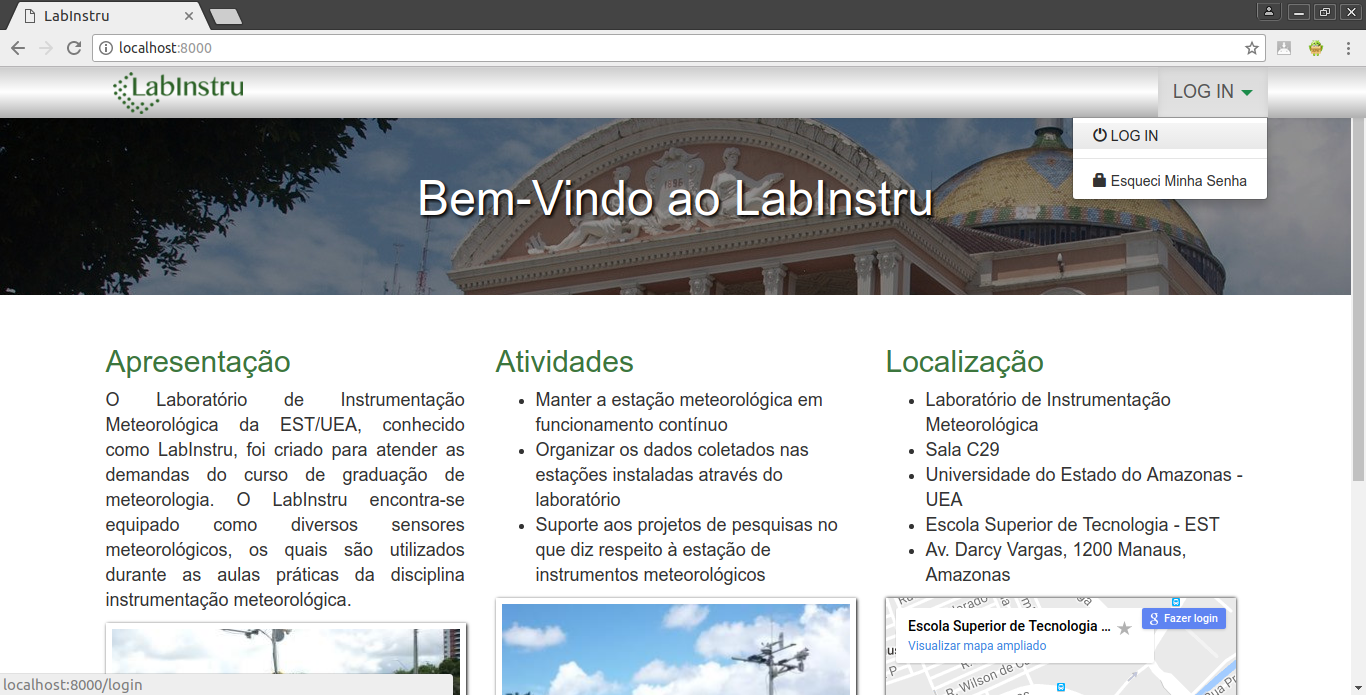
\includegraphics[width=0.9\textwidth]{./img/ap1.png}
	\caption{Página inicial da aplicação LabInstru Web. Fonte: Próprio autor.} \label{fig:ap1}
\end{figure}

\begin{figure}[h!]
	\centering
	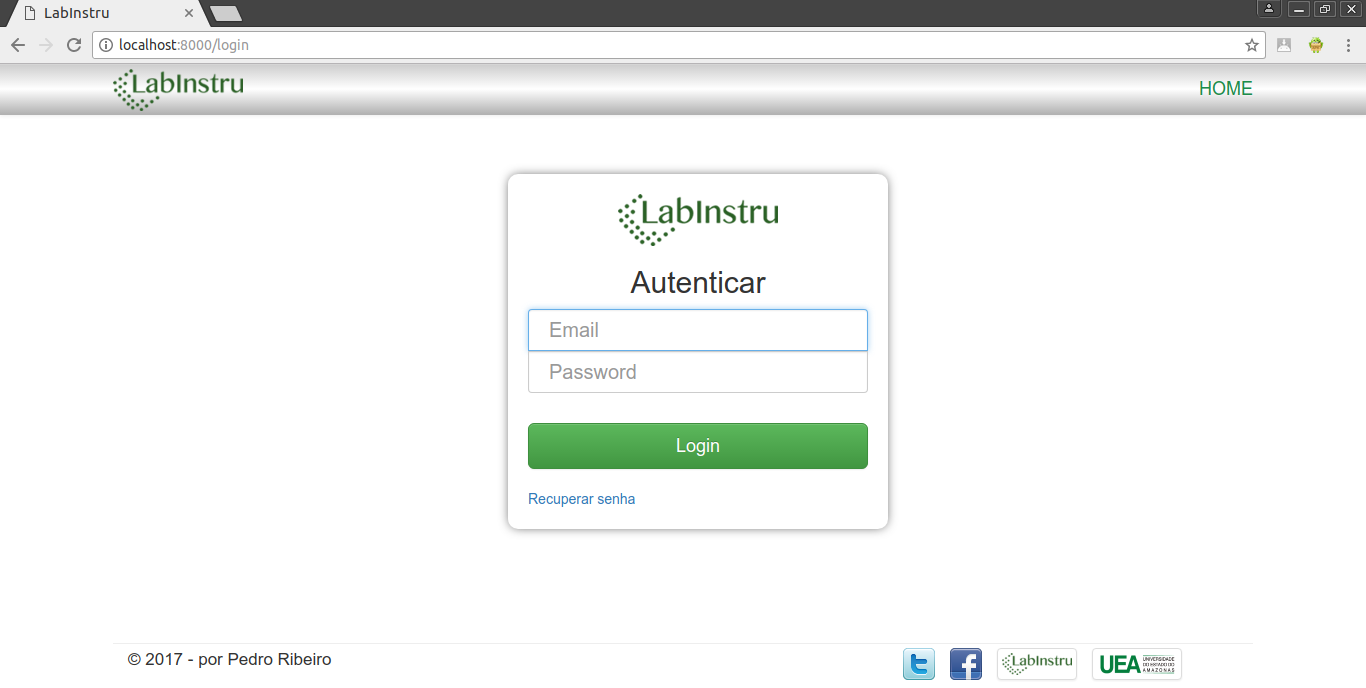
\includegraphics[width=0.9\textwidth]{./img/ap10.png}
	\caption{Formulário de autenticação do sistema. Fonte: Próprio autor.} \label{fig:ap10}
\end{figure}



\begin{figure}[h!]
	\centering
	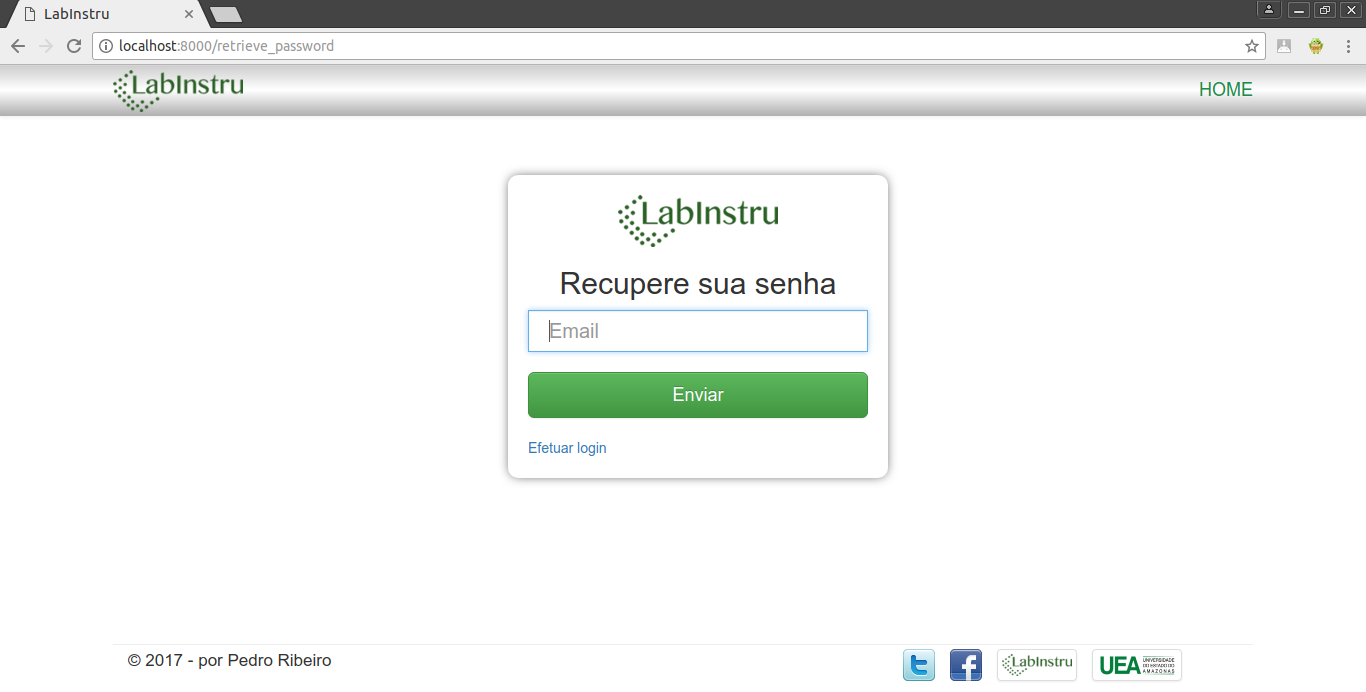
\includegraphics[width=0.9\textwidth]{./img/ap11.png}
	\caption{Formulário para recuperação de senha. Fonte: Próprio autor} \label{fig:ap11}
\end{figure}

A plataforma contempla dois perfis diferentes de acesso: um administrador, a ser desempenhado em termos práticos pela Profa. Maria Betânia Leal, responsável pelo LabInstru, e diversos usuários. O administrador, em especial, é o responsável por fornecer como entrada os dados advindos da estação meteorológica da EST para o LabInstru Web, conforme ilustrado na Figura \ref{fig:ap12}. A aplicação, após processar e persistir os dados advindos da estação, irá fornecer um sumário a respeito do status desta inserção, sob a forma de um \emph{log}. Este \emph{log} exibe quantas medições possuía o arquivo fornecido como entrada, quantas foram corretamente persistidas e quantas resultaram em falha. Um exemplo deste \emph{log} produzido pela aplicação é mostrado na Figura \ref{fig:ap13}.

\begin{figure}[h!]
	\centering
	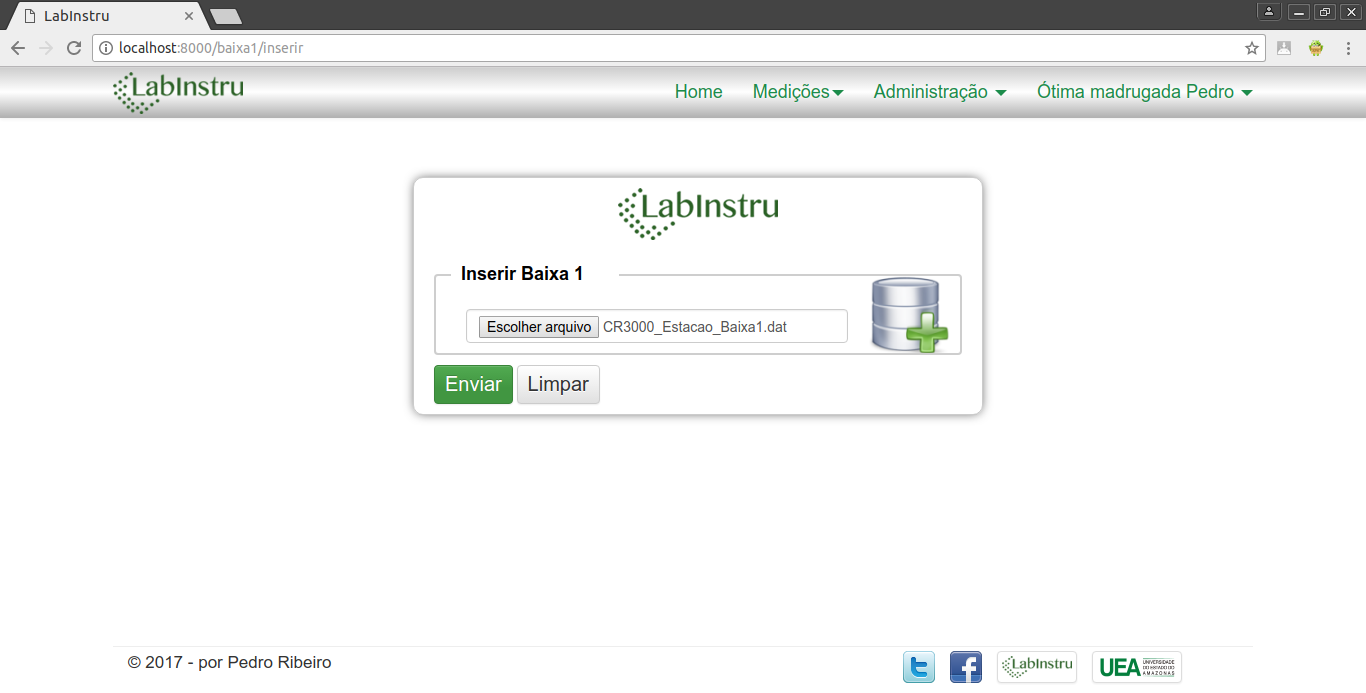
\includegraphics[width=0.9\textwidth]{./img/ap12.png}
	\caption{Página que disponibiliza o formulário para inserção de medições. Fonte: Próprio autor} \label{fig:ap12}
\end{figure}

\begin{figure}[h!]
	\centering
	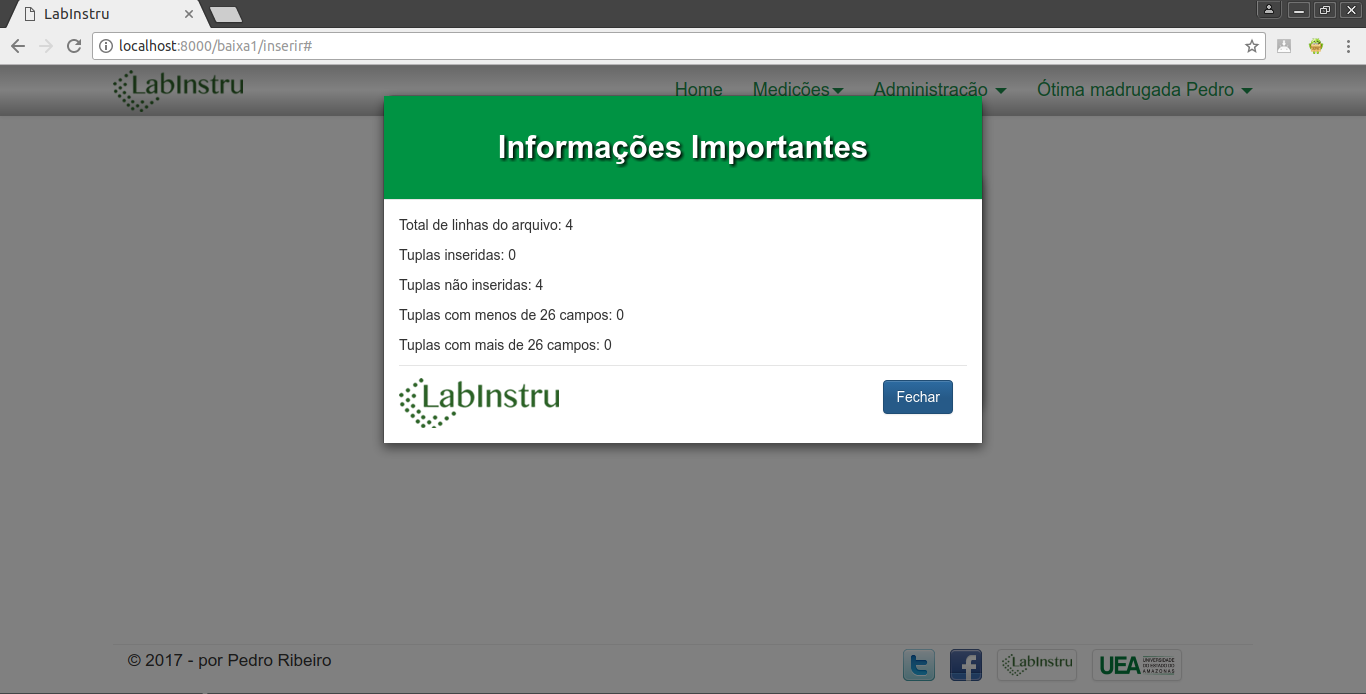
\includegraphics[width=0.9\textwidth]{./img/ap13.png}
	\caption{Exemplo de \emph{log} informando o resultado de uma inserção de medições. Fonte: Próprio autor} \label{fig:ap13}
\end{figure}



O administrador também fica responsável por cadastrar usuários, vide Figura \ref{fig:ap4}, que podem ser alunos de graduação e pós-graduação, outros pesquisadores, docentes, etc. Cabe também ao administrador da aplicação, por meio de uma listagem de usuários disponibilizada pela aplicação, realizar o gerenciamento dos usuários cadastrados na aplicação, conforme ilustrado na Figura \ref{fig:ap14}.

\begin{figure}[h!]
	\centering
	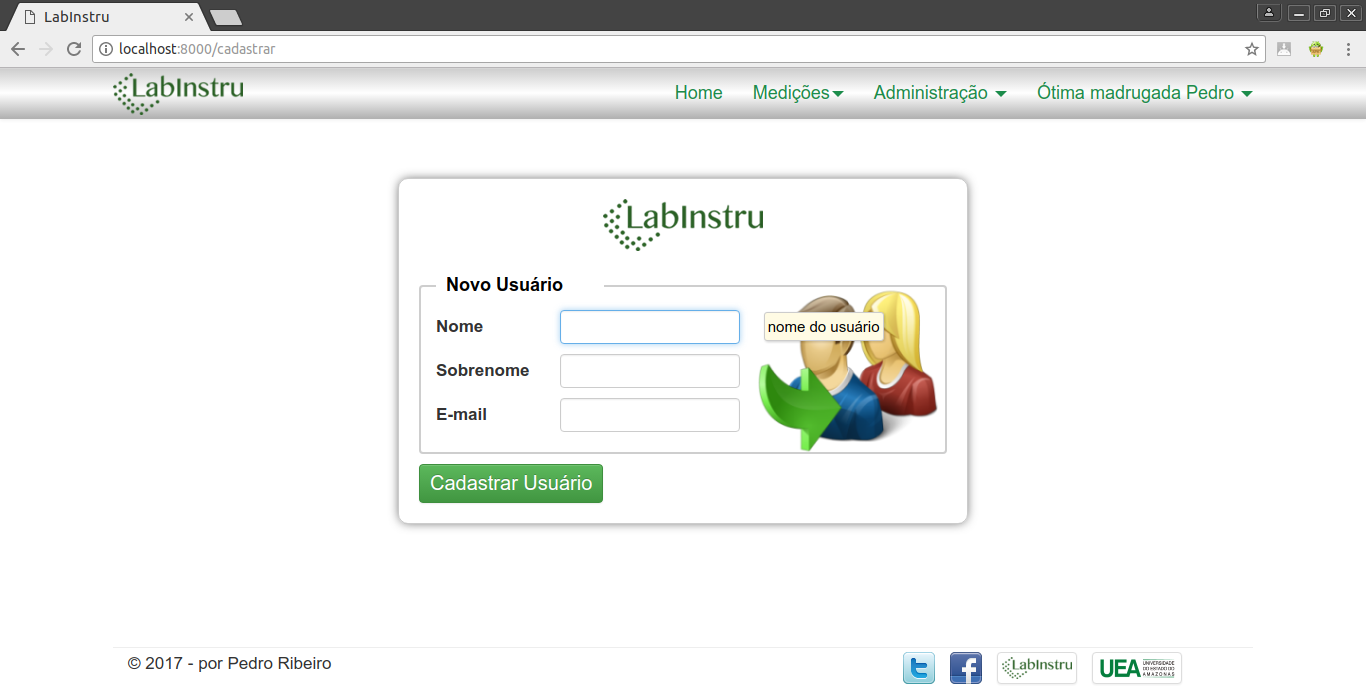
\includegraphics[width=0.9\textwidth]{./img/ap4.png}
	\caption{Página de cadastrado de usuário na plataforma LabInstru Web. Fonte: Próprio autor.} \label{fig:ap4}
\end{figure}

\begin{figure}[h!]
	\centering
	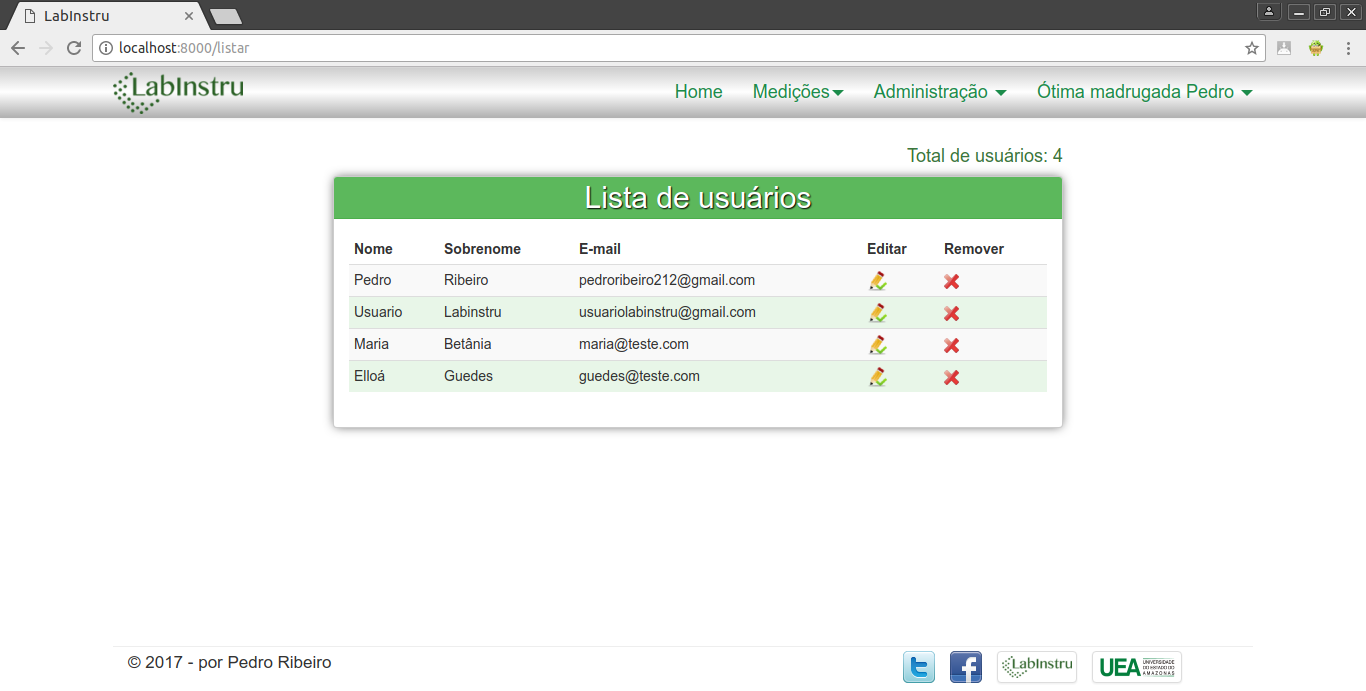
\includegraphics[width=0.9\textwidth]{./img/ap14.png}
	\caption{Lista de usuários cadastrados na aplicação. Fonte: Próprio autor.} \label{fig:ap14}
\end{figure}

Um menu superior, mostrado na Figura \ref{fig:ap1}, permite a autenticação dos usuários e também mostra as principais funcionalidades disponíveis na plataforma após realizada autenticação no sistema. Este menu é renderizado conforme o perfil do usuário. Por exemplo, o menu mostrado ao administrador dispõe da funcionalidade de apagar medições, funcionalidade não disponível no menu mostrado a um usuário. Os menus correspondentes aos diferentes perfis de usuário são ilustrados na Figura \ref{fig:ap8}. Ressalta-se que, independentemente do tipo do perfil de usuário, as principais funcionalidades da plataforma só poderão ser acessadas mediante prévia autenticação na plataforma via login e senha.

\todo{Nova versão da figura, refletindo o novo menu}
\begin{figure}[h!]
	\centering
	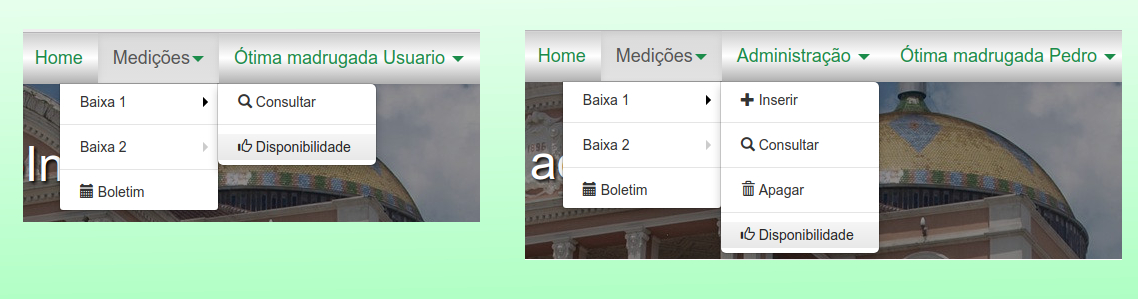
\includegraphics[width=0.9\textwidth]{./img/ap8.png}
	\caption{Exemplos dos menus para diferentes perfis de usuário. Fonte: Próprio autor.} \label{fig:ap8}
\end{figure}

As funcionalidades que permitem a mudança de senha e alteração de seus dados cadastrais são comuns aos dois perfis de usuários. Para ter acesso as mesmas, é necessário apenas que o usuário ou administrador encontre-se autenticado na aplicação. As Figuras \ref{fig:ap5} e \ref{fig:ap6} ilustram, respectivamente, os formulários para mudança de senha e alteração dos dados cadastrais de um determinado usuário (perfil).

\begin{figure}[h!]
	\centering
	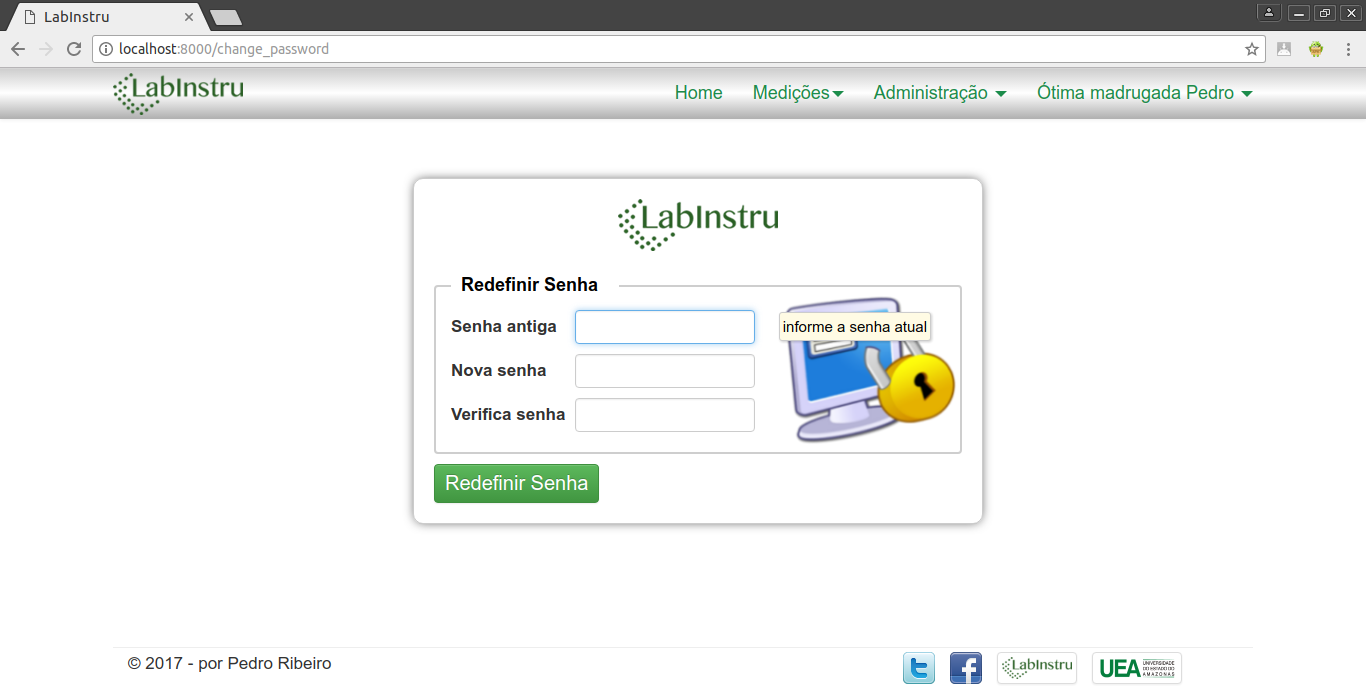
\includegraphics[width=0.9\textwidth]{./img/ap5.png}
	\caption{Formulário para troca de senha. Fonte: Próprio autor.} \label{fig:ap5}
\end{figure}

\begin{figure}[h!]
	\centering
	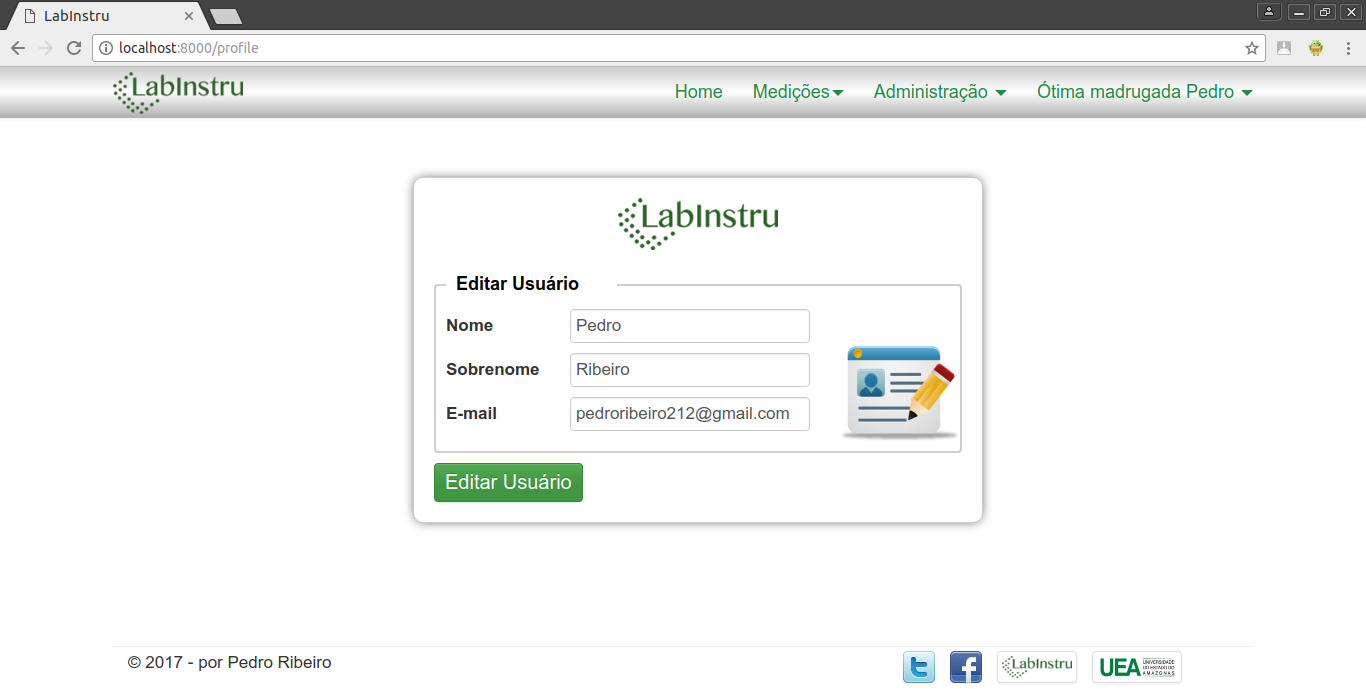
\includegraphics[width=0.9\textwidth]{./img/ap6.png}
	\caption{Página referente a edição de usuário. Fonte: Próprio autor.} \label{fig:ap6}
\end{figure}


Os usuários da plataforma \emph{LabInstru Web} acessam os dados da estação meteorológica da EST por meio de consultas, nas quais fornecem datas iniciais e finais e escolhem as variáveis de interesse, conforme ilustrado na Figura \ref{fig:ap3}. Considerou-se como uma restrição essencial para garantir a integridade e a confiabilidade dos dados que apenas o administrador seria responsável por cadastrá-los.

\todo{Atualizar esta figura}
\begin{figure}[h!]
	\centering
	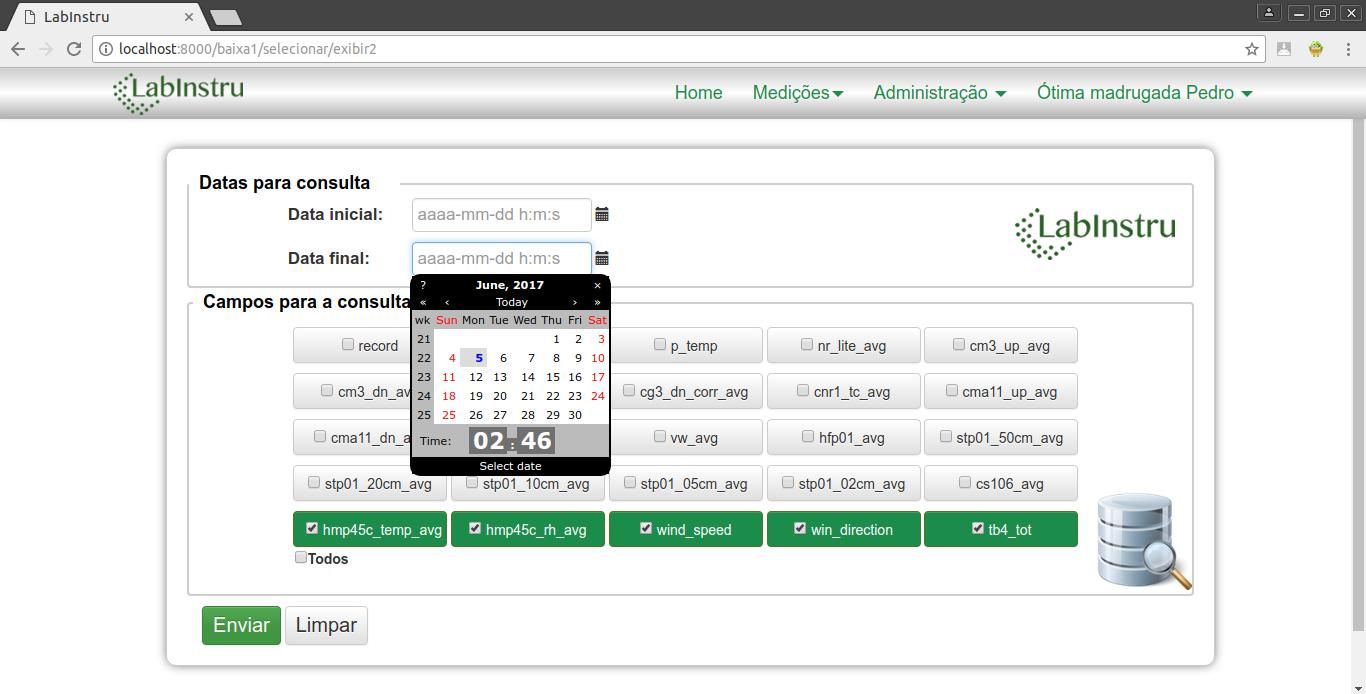
\includegraphics[width=0.9\textwidth]{./img/ap3.png}
	\caption{Página responsável por realizar as consultas. Fonte: Próprio Autor} \label{fig:ap3}
\end{figure}

Os resultados de uma consulta são exibidos em uma página apropriada, onde há opções para exportação dos mesmos nos formatos CSV, HTML, JSON, TSV e XML, conforme ilustra a Figura \ref{fig:ap7}.

\begin{figure}[h!]
	\centering
	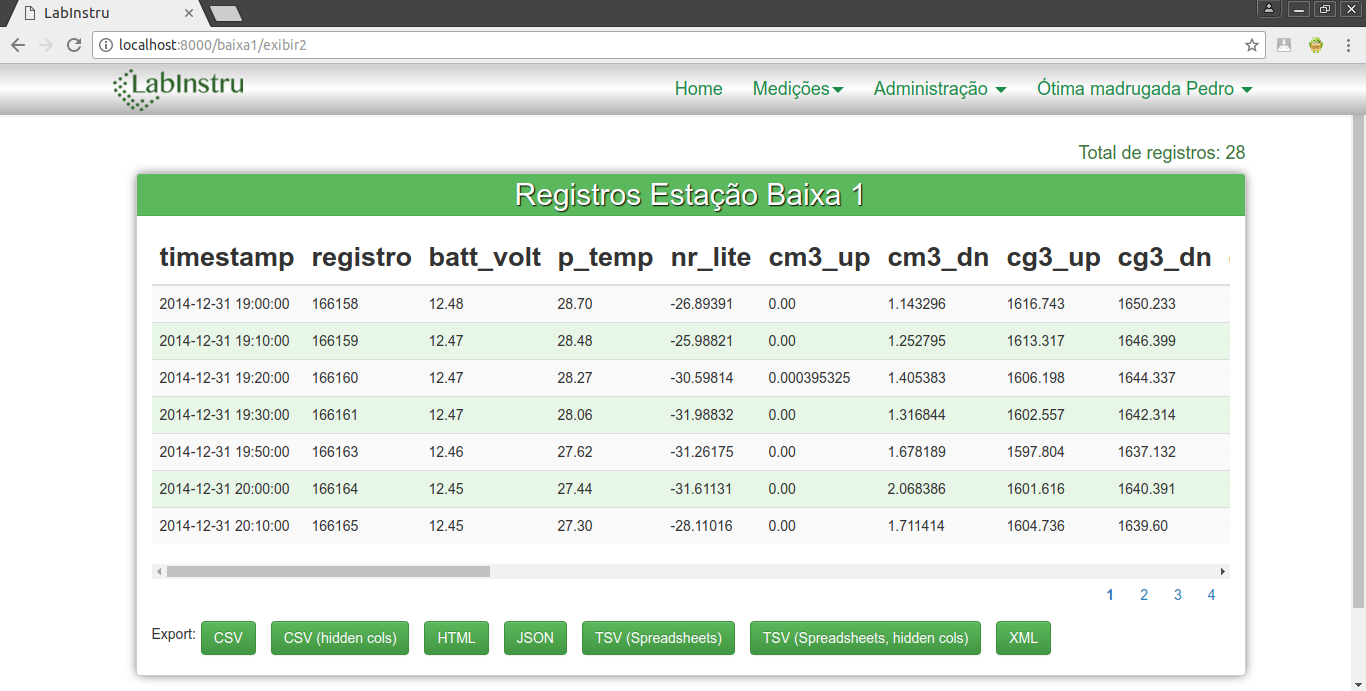
\includegraphics[width=0.9\textwidth]{./img/ap7.png}
	\caption{Página responsável por exibir o resultado de uma consulta. Fonte: Próprio Autor} \label{fig:ap7}
\end{figure}


\section{Implantação da Solução Proposta}

\section{Modelo para Boletim Meteorológico}
Conforme identificado na elicitação de requisitos, uma das funcionalidades requeridas para a plataforma foi a geração de boletins meteorológicos diários, detalhados anteriormente na Seção \ref{sec:boletim}.

Para que esta funcionalidade fosse implementada adequadamente, um melhor refinamento de sua especificação foi necessário, visando a concepção do mesmo, da linguagem visual a ser adotada e dos elementos que deveriam ser incluídos. Como resultado, obteve-se o modelo apresentado na Figura \ref{fig:modeloBoletim}, que contempla a data, precipitação, temperaturas máxima e mínima, índice de calor, rajada e sua classificação na Escala de Beaufort, e ainda a logomarca do LabInstru e da Universidade do Estado do Amazonas.

\begin{figure}[h!]
	\centering
	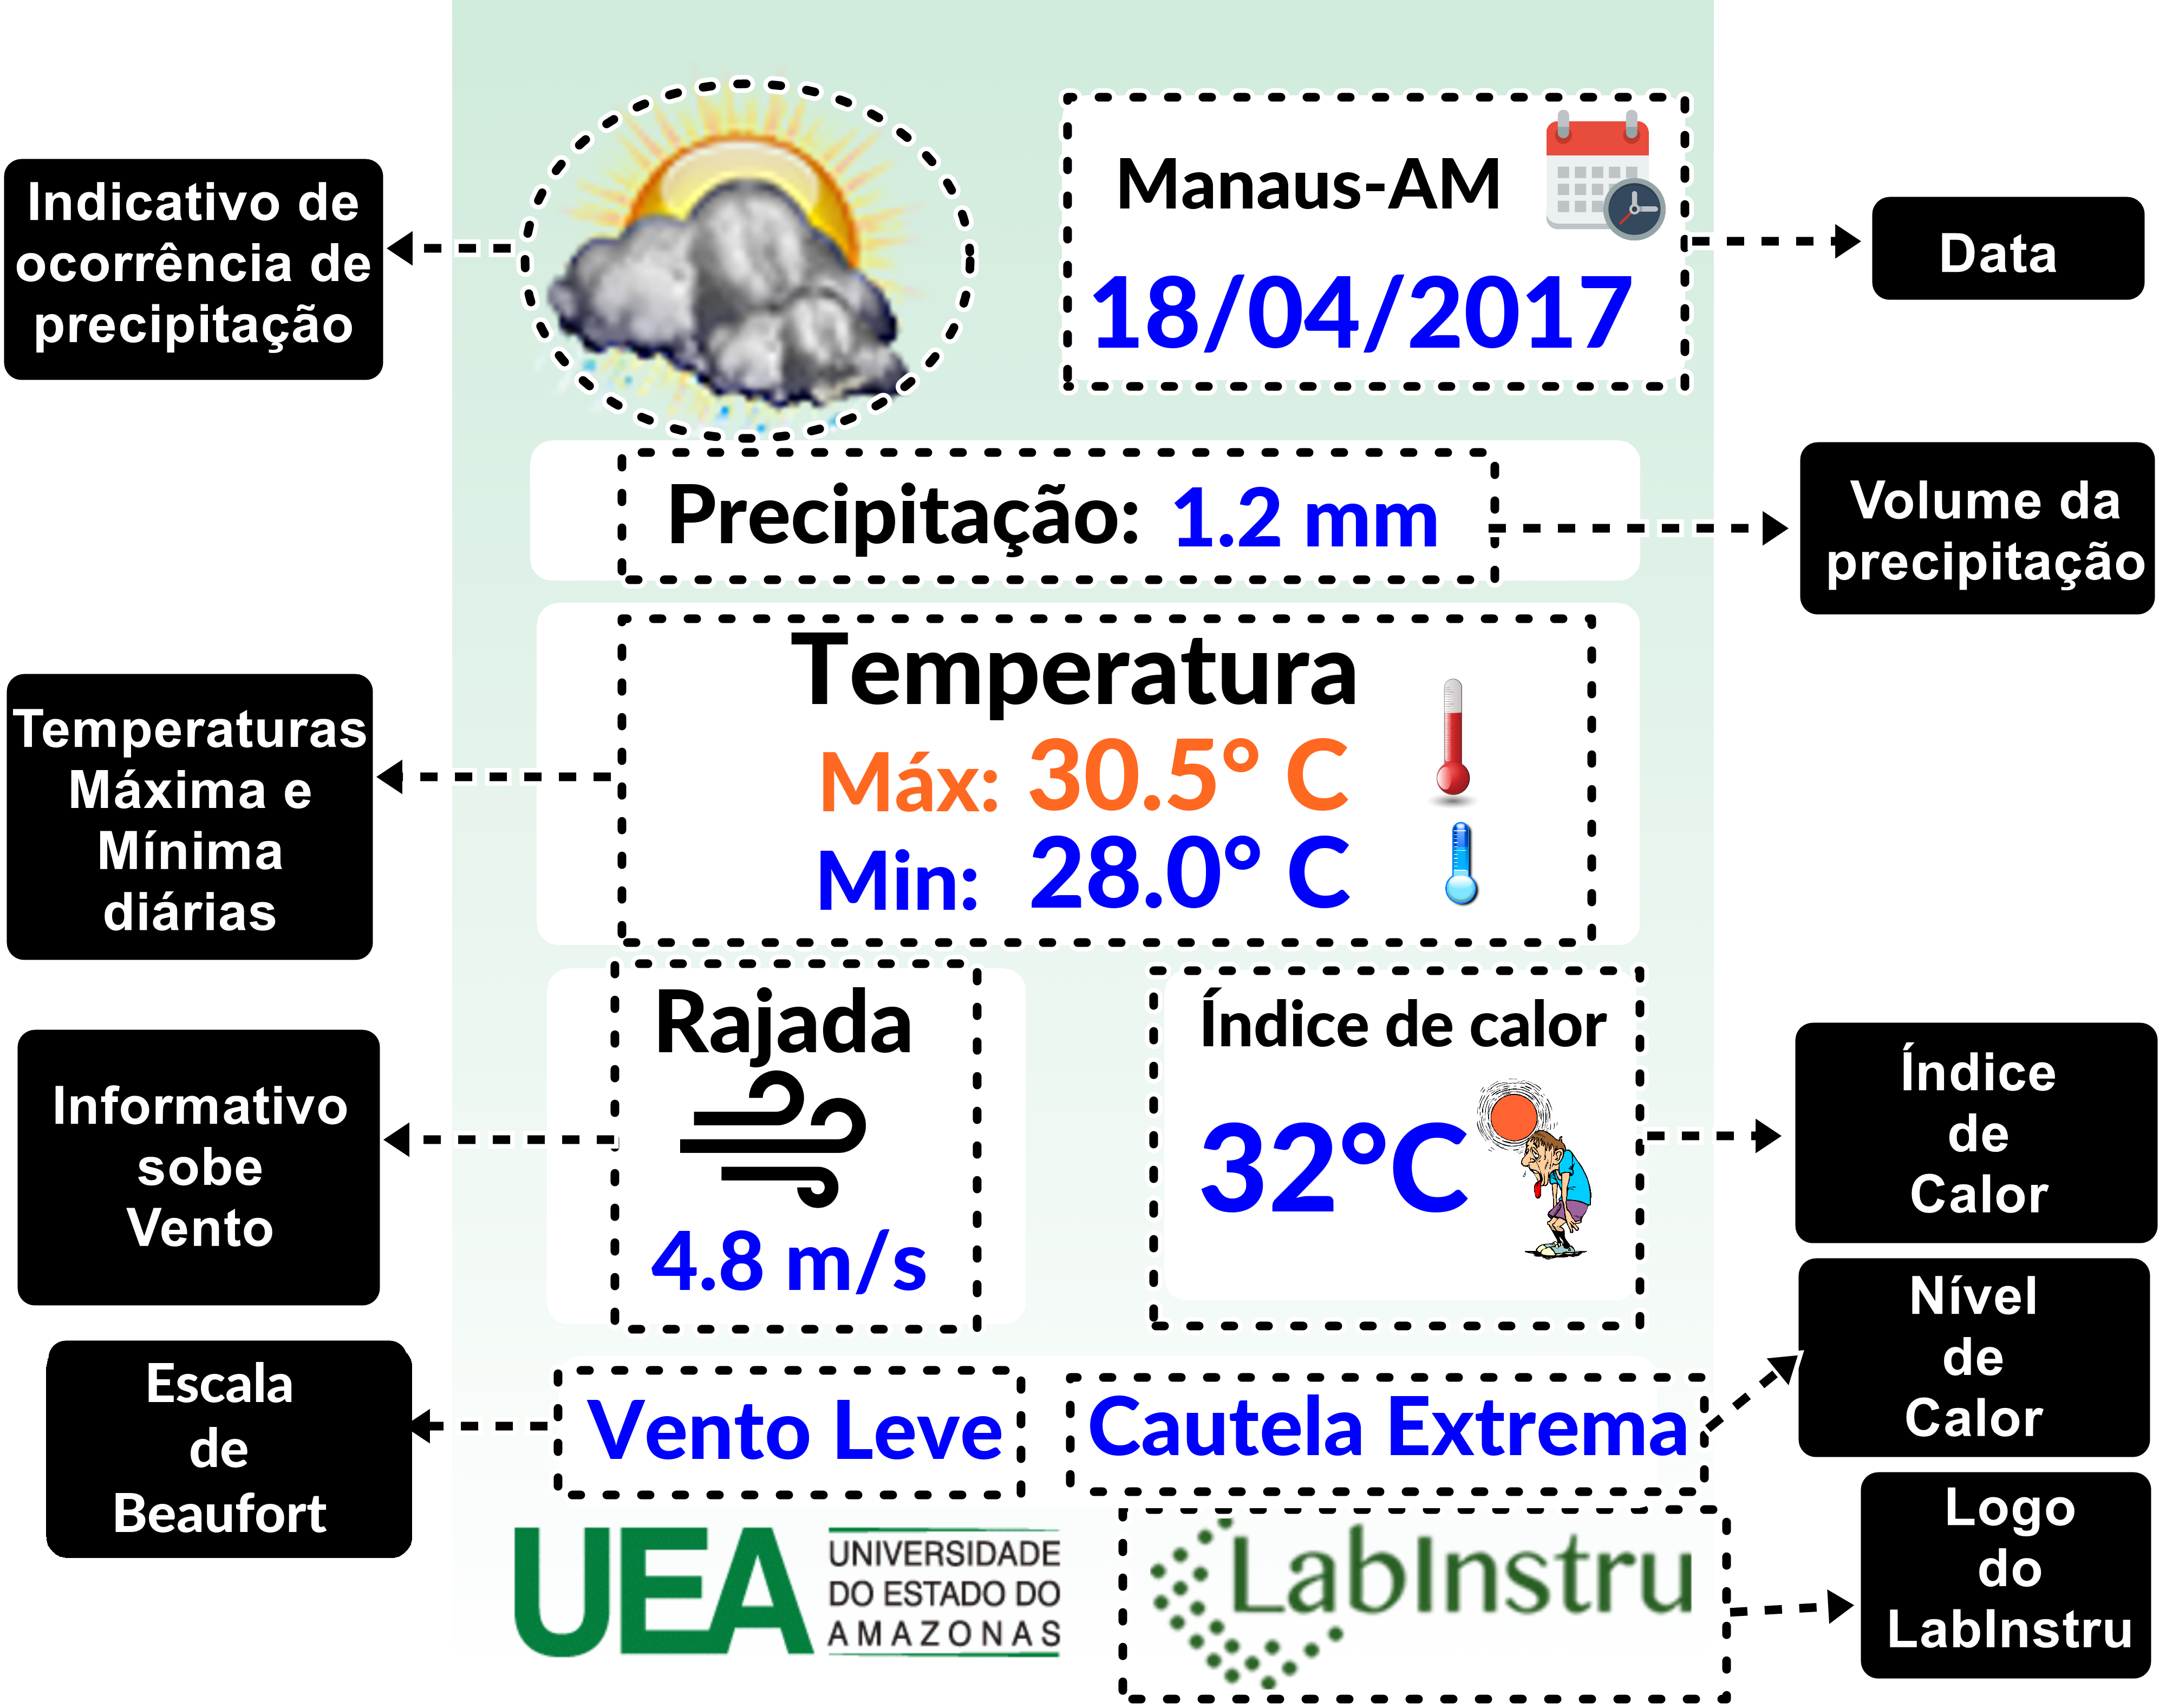
\includegraphics[width=0.5\textwidth]{./img/esbocoBoletim.png}
	\caption{Modelo de referência para boletim meteorológico. Fonte: Próprio autor.} \label{fig:modeloBoletim}
\end{figure}

Para automatizar a geração deste modelo de boletim na solução proposta, foi então necessário implementar o cálculo do índice de calor, desenvolver algoritmos para classificar a rajada e, principalmente, dedicar esforços na interface com o usuário para permitir uma visualização fiel ao modelo discutido com o cliente. Como resultado, o boletim meteorológico produzido com a solução proposta pode ser visto na Figura \ref{fig:boletim}.

\begin{figure}[h!]
	\centering
	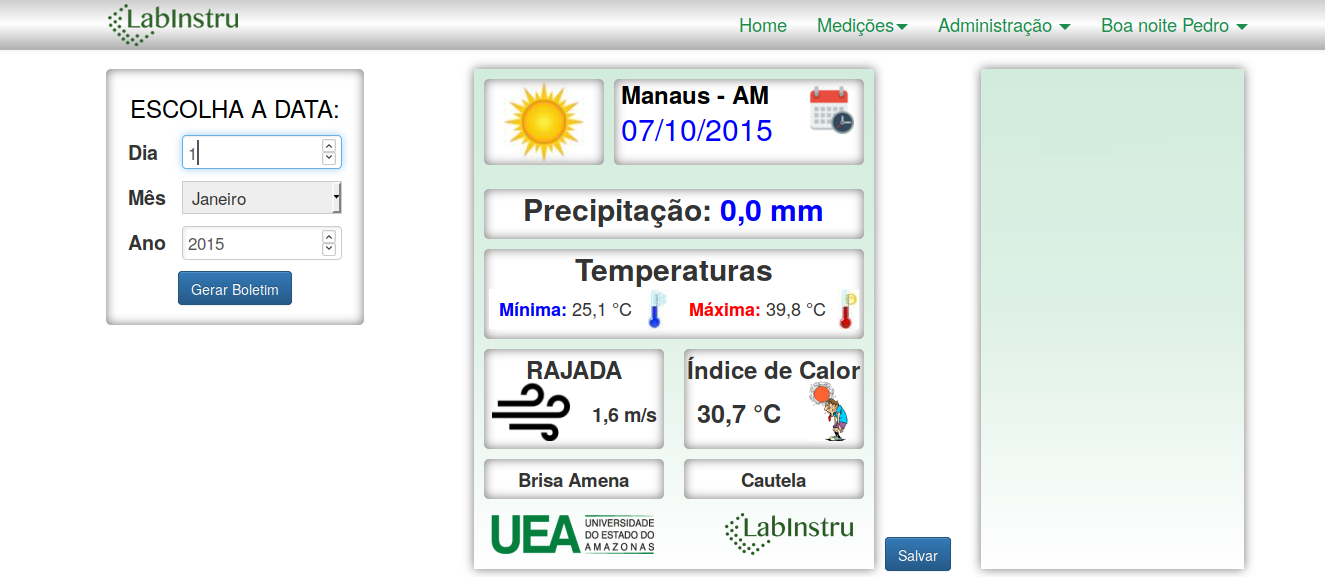
\includegraphics[width=0.9\textwidth]{./img/boletim.png}
	\caption{Boletim meteorológico produzido pelo LabInstru Web. Fonte: Próprio autor.} \label{fig:boletim}
\end{figure}

